\subsection{Distributions of attributes}
Next we are interested in the distributions of the different attributes. In order to evaluate this, histograms are plotted for the attributes 1 to 9. The plots do not include the types, since little new information would be extracted. The histograms are shown in figure \ref{fig:histograms}.

\begin{figure}[H]
\centering
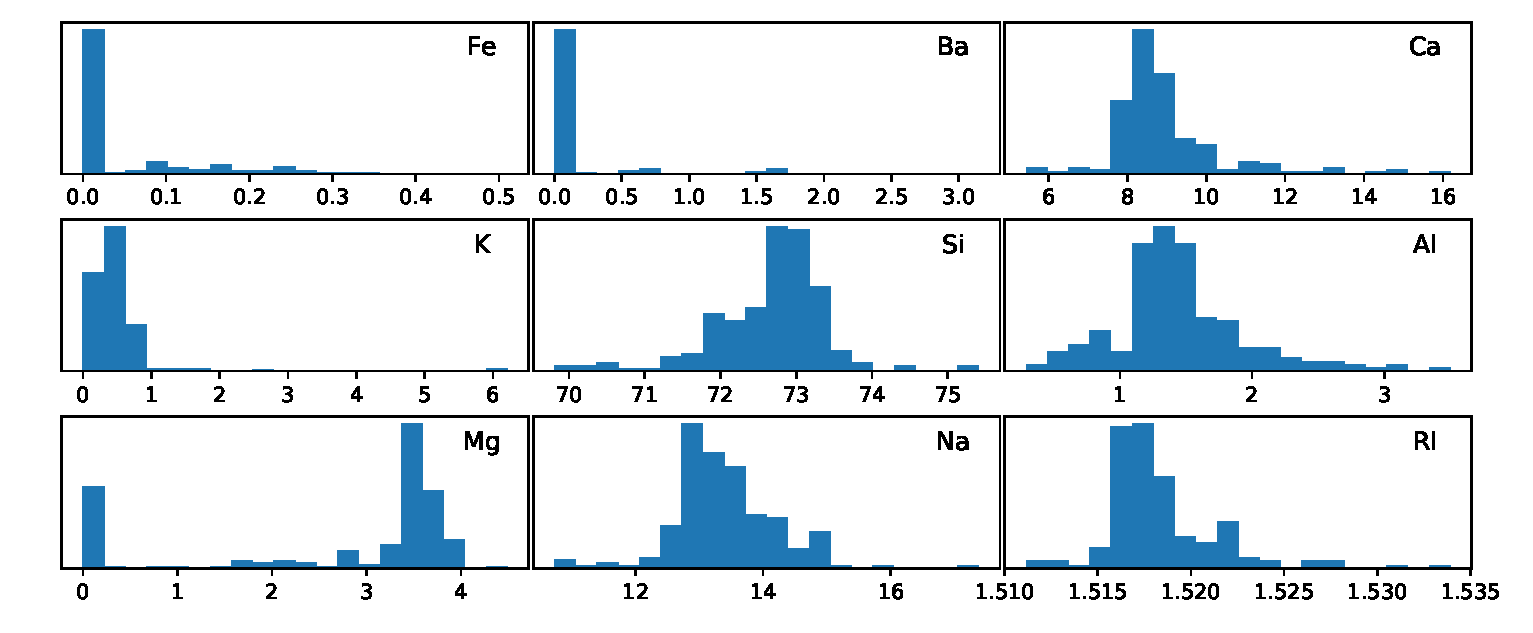
\includegraphics[width=1\linewidth]{fig/HistogramAll.eps} 
\caption{Histogram of all attributes except glass type.}
\label{fig:histograms}
\end{figure}

From the shown 9 attributes of the data set, \texttt{RI}, (\texttt{Na}), \texttt{Al}, \texttt{Si} and \texttt{Ca} are the ones that follow a normal distribution the most. Attributes such as \texttt{Fe}, \texttt{Ba}, \texttt{K} follow what looks more like a logarithmic distribution, while \texttt{Mg} looks multimodal. The tendency to be left skewed, might be explained intuitively given that the attributes mostly describe contents. When the majority of the observations contain little to no content of the last 4 mentioned constituents, but for occasional peaks in content, we get a left skewed distribution with a tail to the right.